Conforme dito no capítulo \ref{chap:mati}, o trabalho foi dividido em 4 etapas, nas quais a primeira etapa consistiu no estudo dos DPDs e nos métodos de modelagem deles, a segunda etapa consistiu na implementação desta modelagem em software, a qual utilizou-se o python, a etapa 3 que consiste na implementação do modelo de DPD escolhido em hardware utilizando a linguagem VHDL e finalmente na quarta etapa é feita o design do circuito integrado.
Neste capítulo sãi exibidos os resultados da etapa 2 já que a etapa 1 consiste na pesquisa bibliográfica e as etapas 3 e 4 serão desenvolvidas na segunda etapa do projeto.

\section{Modelagem do PA}

Para fazer a modelagem em software foi utilizada a linguagem de programação Python. Para isso, separou-se os dados citados na seção \ref{sec:implsoft} do capítulo \ref{chap:mati}, em dados de extração e dados de validação, os quais são utilizados para extração dos coeficientes do modelo do MP e validação do modelo encontrado, respectivamente. Para fazer a validação do modelo utilizou-se a métrica do NMSE, que consiste em calcular o erro médio quadrado do valor medido pelo VSA para o valor calculado pelo modelo. Portanto, quanto menor o NMSE mais fiel é o modelo do PA. Nesta etapa obteve-se um NMSE de -23.57 dB, para cálculos em virgula flutuante, onde o resultado está presente no gráfico da figura \ref{fig:modelopafloat}.

\begin{figure}[ht!]
    \centering
    \captionsetup{justification=centering}
    \caption*{Fonte: Autor}
    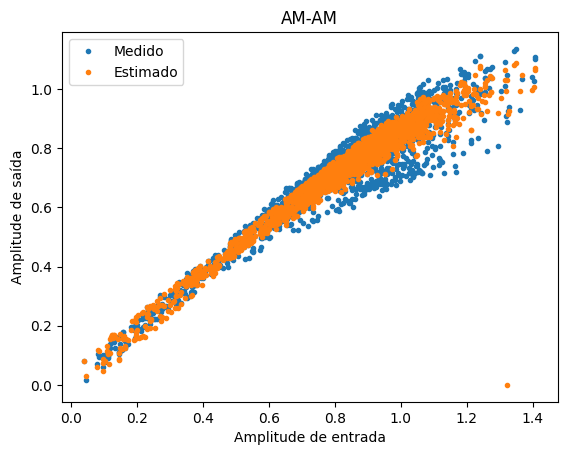
\includegraphics[width=\figsize]{modeloPAfloat.png}
    \caption{Modelo do PA em vírgula flutuante}
    \label{fig:modelopafloat}
\end{figure}

\section{levantamento do número de bits}

Após concluída a modelagem matemática, foi feita a modelagem do DPD para então ser feito o levantamento da quantidade de bits necessários para a implementação do DPD em hardware minimizando os erros de quantização. 
Para isso foi necessário refazer a extração dos coeficientes, mas desta vez com os dados normalizados para valores de 0 a $2^{bits}$.  
O resultado desse levantamento está presente no gráfico na figura \ref{fig:bits}.

\begin{figure}[ht!]
    \centering
    \captionsetup{justification=centering}
    \caption*{Fonte: Autor}
    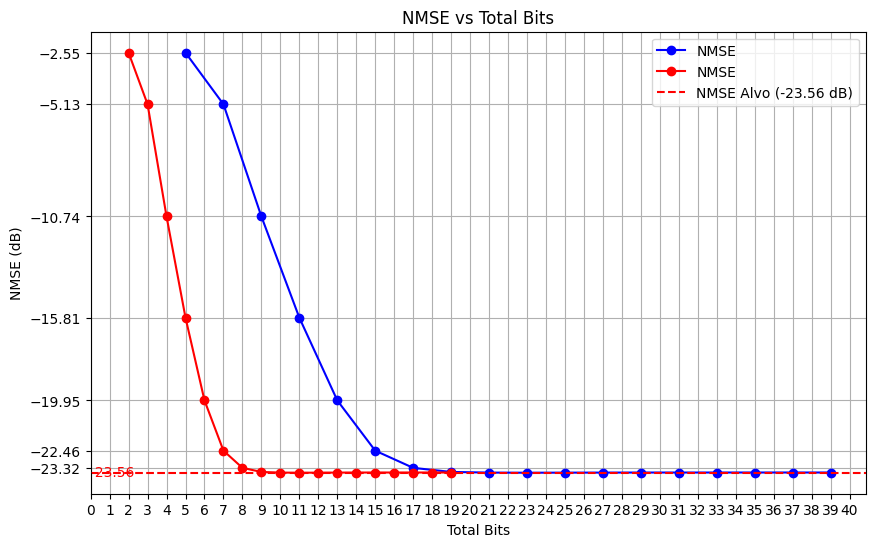
\includegraphics[width=\figsize]{bits.png}
    \caption{Gráfico Número de bits x NMSE}
    \label{fig:bits}
\end{figure}

Neste gráfico observa-se duas curvas, a curva em azul apresenta a quantidade total de bits total contando com os bits de overflow necessárias para as operações de multiplicação, enquanto a curva em vermelho representa a quantidade de bits de resolução do sinal. Analisando este gráfico observou-se que não existem ganhos significativos no erro a partir de 7 bits, portanto foi feita a modelagem do PA utilizando uma resolução de 8 bits o resultado alcançado está ilustrado pela figura \ref{fig:modelopa}.

\begin{figure}[ht!]
    \centering
    \captionsetup{justification=centering}
    \caption*{Fonte: Autor}
    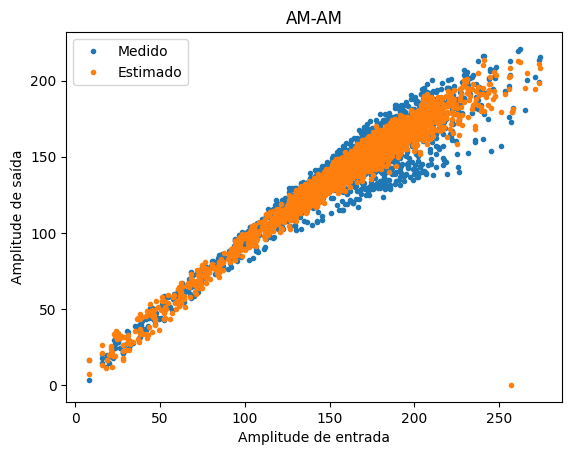
\includegraphics[width=\figsize]{modeloPA.png}
    \caption{Modelo do PA em vírgula fixa}
    \label{fig:modelopa}
\end{figure}

\section{Modelagem do DPD}
A partir dos resultados obtidos foi possível fazer a modelagem do DPD, para isso foi feito o mesmo processo de modelagem do PA, porém para alcançar a característica de transferência inversa PA foi invertido a ordem dos dados de entrada e saída para extração dos coeficientes do DPD. O resultado desta modelagem está ilustrado pela figura \ref{fig:modelodpd} a seguir.

\begin{figure}[ht!]
    \centering
    \captionsetup{justification=centering}
    \caption*{Fonte: Autor}
    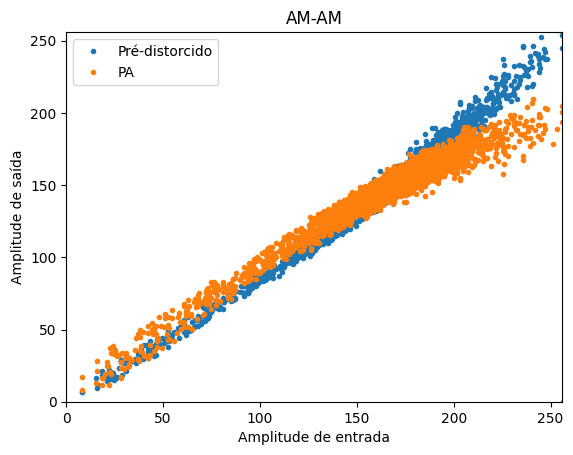
\includegraphics[width=\figsize]{modelodpd.png}
    \caption{Modelo do DPD em vírgula fixa}
    \label{fig:modelodpd}
\end{figure}